\documentclass{article}
\usepackage{amsmath,amssymb}
\usepackage{tikz}
\usetikzlibrary{arrows.meta,positioning,calc,shapes.geometric}
\pagestyle{empty}
\begin{document}
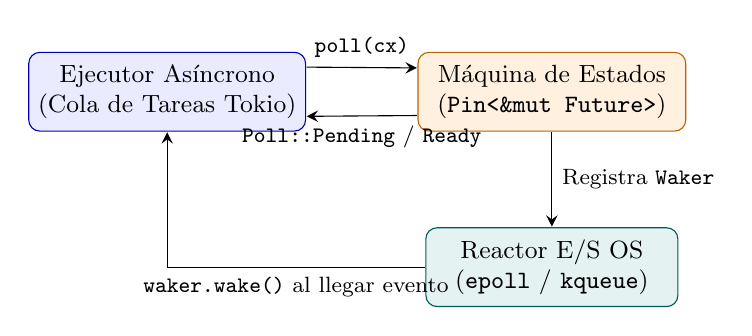
\begin{tikzpicture}
\tikzset{node distance=2.2cm, >=stealth, thick, font=\small}
\node[draw=blue!70!black, fill=blue!8, rounded corners, minimum width=3.2cm, minimum height=1.0cm, align=center] (exec) {Ejecutor Asíncrono\\(Cola de Tareas Tokio)};
\node[draw=orange!75!black, fill=orange!12, rounded corners, minimum width=3.4cm, minimum height=1.0cm, align=center, right=1.4cm of exec] (fut) {Máquina de Estados\\(\texttt{Pin<\&mut Future>})};
\node[draw=teal!70!black, fill=teal!10, rounded corners, minimum width=3.2cm, minimum height=1.0cm, align=center, below=1.2cm of fut] (reac) {Reactor E/S OS\\(\texttt{epoll} / \texttt{kqueue})};
\draw[->] (exec.10) -- node[above, font=\footnotesize] {\texttt{poll(cx)}} (fut.170);
\draw[<-] (exec.350) -- node[below, font=\footnotesize] {\texttt{Poll::Pending} / \texttt{Ready}} (fut.190);
\draw[->] (fut) -- node[right, font=\footnotesize] {Registra \texttt{Waker}} (reac);
\draw[->] (reac.west) -| node[pos=0.25, below, font=\footnotesize] {\texttt{waker.wake()} al llegar evento} (exec.south);
\end{tikzpicture}
\end{document}
